\section{Constructing blockchain proofs}

Based on the model we introduced previously, we now move on to provide a
concrete non-interactive PoPoW construction which allows proving certain
predicates $Q$ of the chain $\chain$. Among the predicates which are stable, we
limit ourselves to the class of predicates which are functions of only the
chain suffix $\chain[:-k]$. As we will illustrate, these predicates are
significantly easier to prove, but at the same time seem to be the most useful
class of predicates which one needs for applications.

Specifically, these predicates allow proving that a transaction occurred in the
longest chain and in a block burried under $k$ blocks, which is sufficient for
verifying payments in the SPV case. Furthermore, these predicates are
expressive enough to describe the inclusion of the specific transactions needed
for building sidechains.

The \textsc{Verify} function of our NIPoPoW construction is described in
Algorithm~\ref{alg.nipopow-verifier}.

\import{./}{algorithms/alg.verifier-lite.tex}

We introduce a helper algorithm, constructInnerChain, shown in
Algorithm~\ref{alg.nipopow-innerchain}. This algorithm returns the innerchain
of level $i$ extracted from the blockchain $\chain$. If boundary is provided,
it only returns the blocks more recent than the boundary block supplied.

\import{./}{algorithms/alg.nipopow-prover.tex}
\import{./}{algorithms/alg.nipopow-innerchain.tex}

The NIPoPoW proof construction is shown in Algorithm~\ref{alg.nipopow-construct-proof}.
This produces a non-interactive PoPoW in parameter $m$ which consists of a
number of blocks for every level $i$. The number of blocks per level is
approximately $2m$.

\begin{figure}[h]
    \caption{The hierarchical blockchain. Existing blocks are shown in level 1.
    Higher levels have achieved a lower target (higher difficulty) during mining.}
    \centering
    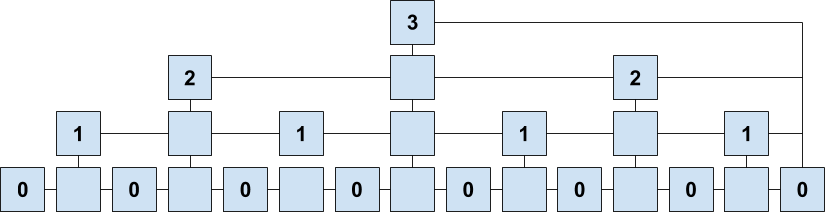
\includegraphics[width=0.5\textwidth,keepaspectratio]{figures/hierarchical-ledger.png}
    \label{fig:hierarchy}
\end{figure}

\begin{figure}[h]
    \caption{The first of a series of interactive proofs-of-proofs-of-work for
    $m = k = 3$. This proof is the only one that needs to be sent in case it
    goes unchallenged.}
    \centering
    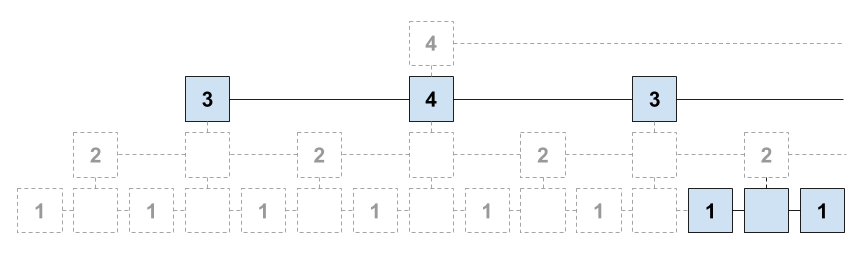
\includegraphics[width=0.5\textwidth,keepaspectratio]{figures/interactive-popow.png}
\end{figure}

\begin{figure}[h]
    \caption{A non-interactive proof-of-work for $m = k = 3$. Any challenges
    can be answered by the verifier directly by constructing a proof from the
    data in this proof, without interaction with the prover.}
    \centering
    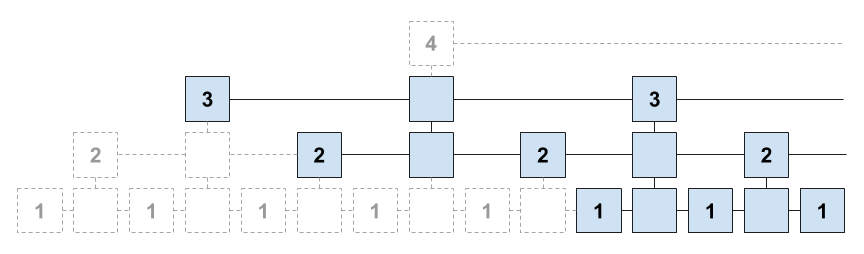
\includegraphics[width=0.5\textwidth,keepaspectratio]{figures/non-interactive-popow.png}
\end{figure}

\import{./}{algorithms/alg.nipopow-maxchain.tex}
